
% this file is called up by thesis.tex
% content in this file will be fed into the main document
% ----------------------- paths to graphics ------------------------

% change according to folder and file names
\ifpdf
    \graphicspath{{8/figures/PNG/}{8/figures/PDF/}{8/figures/}}
\else
    \graphicspath{{8/figures/EPS/}{8/figures/}}
\fi


\chapter{Regulated hydraulic turbines.}

In order to increase the hydraulic turbine operational flexibility, in terms of variation in flowrate (Q) and hydraulic head (H), the concept of regulation is used. A regulated hydraulic turbine is a turbine with adjustable blades, either stator or rotor or both. An adjustable blade is a blade that can be rotated around a predefined axis through a appropriately designed mechanism. 


\section{Single-regulated turbines}
\label{single.regulated}

Hydraulic turbines that have only one set of adjustable blades (usually these are the stator blades) are called single-regulated turbines (see figure \ref{signle}). Typical examples of this type are: Francis turbines, axial fixed-blade propeller turbines with adjustable stator blades and the so called semi-Kaplan concept where fixed stator blades and adjustable rotor blades are used \cite{Papanto,drtina1999hydraulic}.  
Although the rotation angle of the adjustable blades ($\alpha$) for each operating point could be treated as additional design variables, one per operating point, a different approach is proposed in this thesis. 
                 

\begin{figure}[h!]
\centering
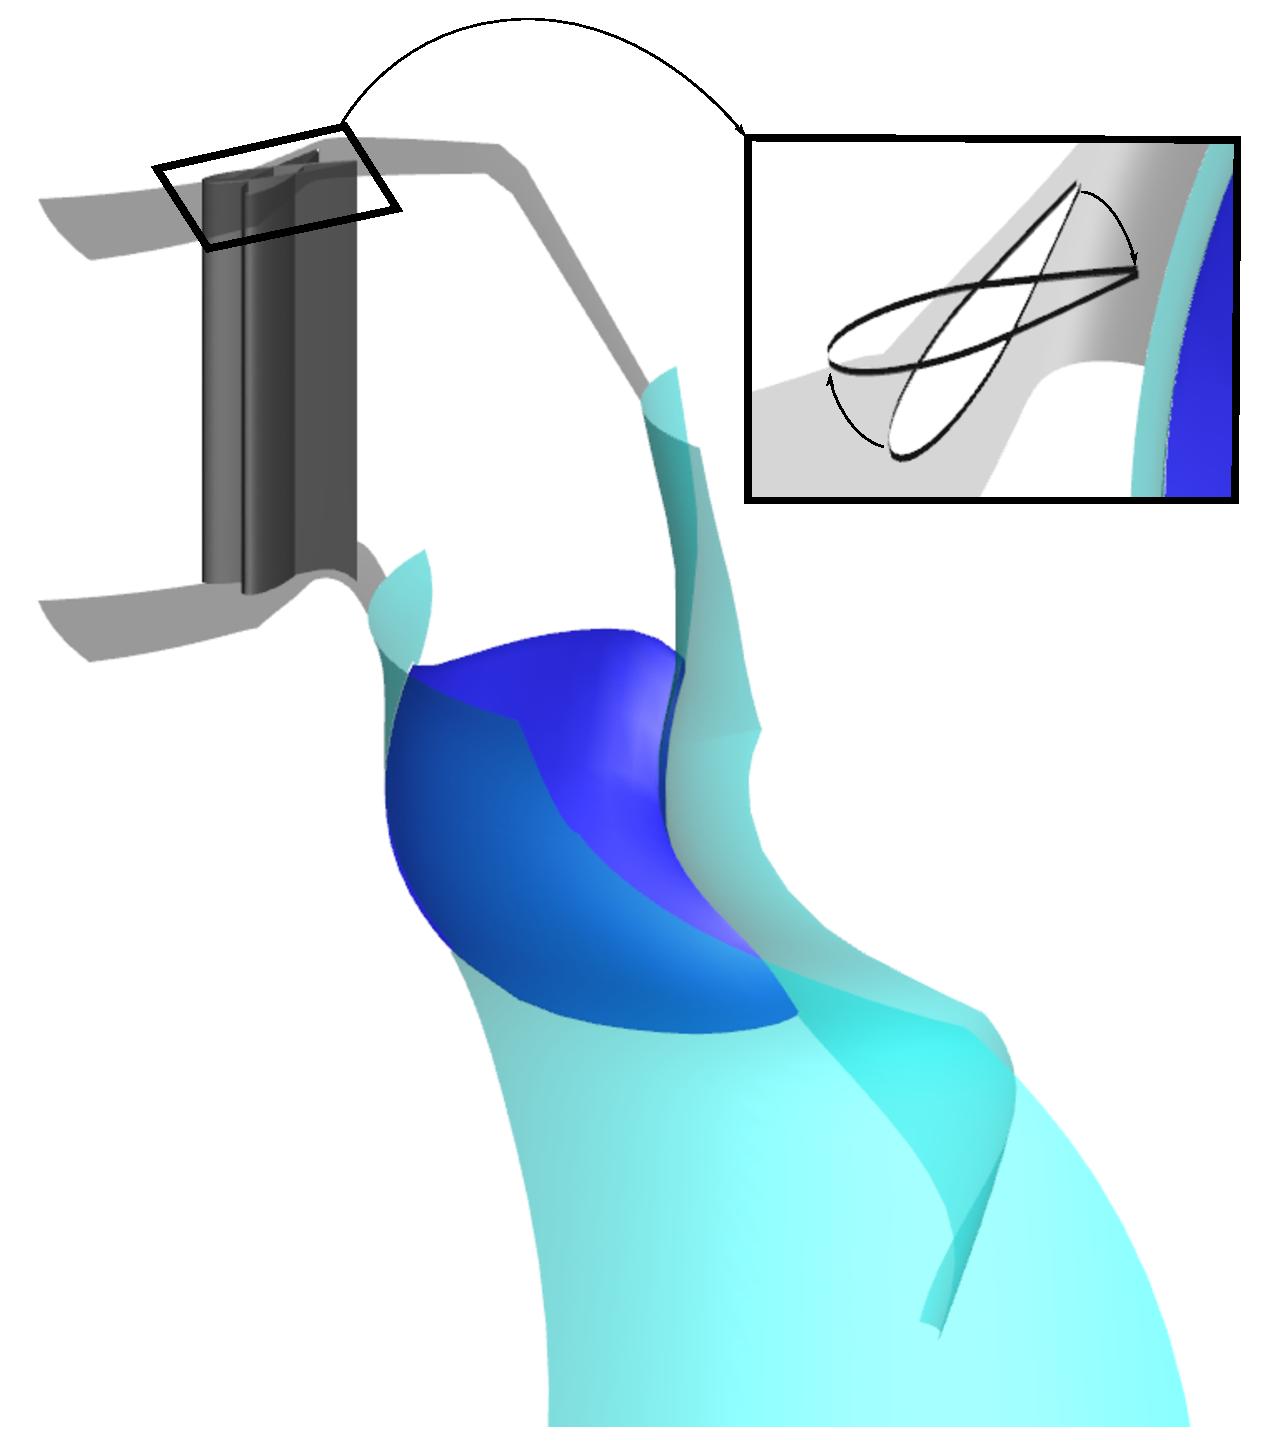
\includegraphics[width=.8\textwidth]{SINGLE.eps}
\caption{Single-regulated turbine.}
\label{signle}
\end{figure}


Regarding the single-regulated turbine problem, the proposed method aims at eliminating the need of additional constraints so as to ensure operation at the desirable operating point. This is achieved by ensuring that each candidate solution will operate at the appropriate $\alpha$ so as to operate at the desirable operating point. Should this be the case, then the quality metrics are computed and the evolution continuous as presented before. 

The proposed approach takes place by enhancing the candidate solution evaluation procedure so at to calculate the appropriate $\alpha$ for the desirable operating point. This is achieved through the algorithm presented below. 
\newpage
For each candidate solution:
\begin{itemize}
\item[]{\bf Step 1:}  (Initialization) 
\begin{itemize}
	\item[]{\bf Step 1a:} (Initial $\alpha$) Set the iteration counter to $i=0$ and $\alpha_i=\alpha _0$, where $\alpha _0$ a user defined value.
	\item[]{\bf Step 1b:} (First step) Set $i=1$ and $\Delta \alpha= \Delta \alpha_0$ where $\Delta \alpha_0$ the user-defined increment. Perform the first step:
\begin{eqnarray}
	\alpha_1={\left\{ 
	\begin{array}{ll}
    \alpha_0 - \Delta \alpha_0 ~~,\mbox{if $(Q < Q_{required})$ or ($H > H_{required})$}\\
	\alpha_0 + \Delta \alpha_0 ~~,\mbox{if $(Q > Q_{required})$ or $(H < H_{required})$}\\
    \end{array} \right. }
    \label{step0}
\end{eqnarray}  
It is reminded that $\alpha=0^o$ corresponds to the fully open stator position.
\end{itemize}

\item[]{\bf Step 2:}  (Gradient computation) Set $i=i+1$. Compute the gradient of either $\frac{\partial(Q-Q{required})}{\partial \alpha}$ or $\frac{\partial(H-H{required})}{\partial \alpha}$, depending on the chosen boundary conditions of the solver in hand. The two variations are identical. Herein the Q example will be used for space economy. 
\begin{eqnarray}
	\frac{\partial(Q-Q_{required})}{\partial \alpha}=\frac{(Q_{i-1}-Q_{required})-(Q_{i-2}-Q_{required})}{\alpha_{i-1}- \alpha_{i-2}}
\end{eqnarray}  

\item[]{\bf Step 3:}  (Update $\alpha$) Based on the Newton-Raphson method the $\alpha$ can be updated as follows
\begin{eqnarray}
	\alpha_{i}=\alpha_{i-1} - \eta \frac{Q_{i-1}-Q_{required}} {\frac{\partial(Q-Q_{required})}{\partial \alpha}}  
\end{eqnarray}  
where $\eta$ a user defined relaxation factor. 

\item[]{\bf Step 3:} (Convergence check) If $|Q_{i}-Q_{required}|<\Delta Q^*$ Stop else go to step 2. Where $\Delta Q^*$ a user defined threshold value.
\end{itemize}  

This algorithm can be scaled to any number of operating points for handling multi operating point design problems.     

\section{Double-regulated turbines}

Hydraulic turbines that have two sets of adjustable blades (rotor and stator) are called double-regulated turbines (see figure \ref{double}). Typical examples of this is the Kaplan turbine.  
Herein the angle of rotation of the adjustable stator blades is denoted as $\alpha$ (in accordance with the previous section) and of the rotor blades as $\beta$. Furthermore, apart from the operation in the desirable operating point, the $C_u$ velocity component at the outlet of the runner at the hub position is required to have the user-defined (through the target $C_u$ distribution) value, the second requirement is denoted as $S$.     
Regarding the operating point requirement, the Q variation will be used as before, having in mind that it could easily be transformed to the H one.  

\begin{figure}[h!]
\centering
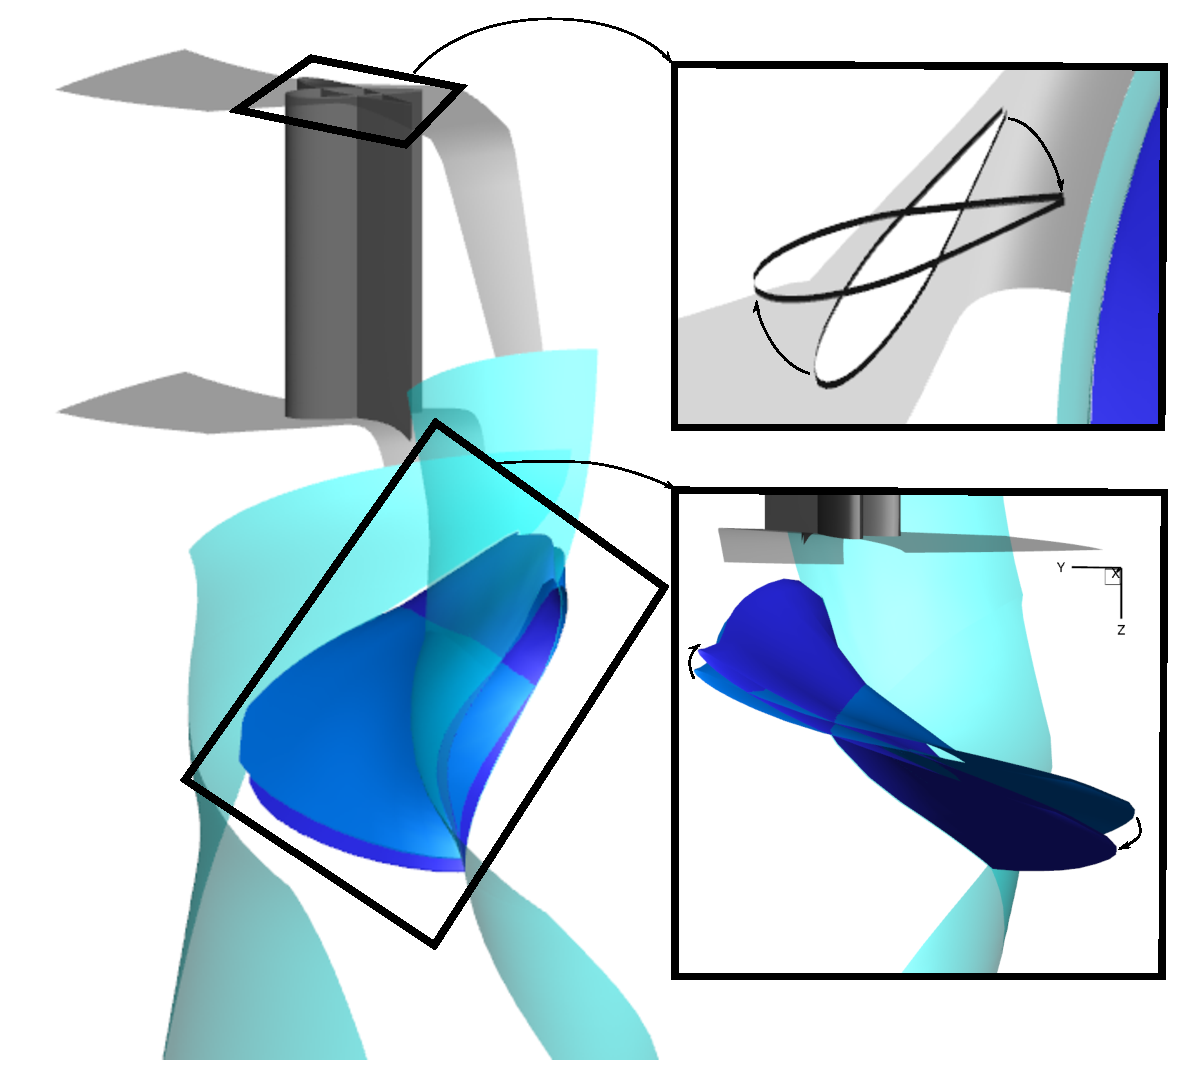
\includegraphics[width=.8\textwidth]{DOUBLE.eps}
\caption{Double-regulated turbine.}
\label{double}
\end{figure}


The algorithm of the approach suitable for double-regulated turbines follows.
For each candidate solution:
\begin{itemize}
\item[]{\bf Step 1:}  (Initialization) 
\begin{itemize}
	\item[]{\bf Step 1a:} (Initial $\alpha$ and $\beta$) Set the iteration counted to $i=0$, $\alpha_i=\alpha _0$ and $\beta_i=\beta _0$ where $\alpha _0$ and $\beta _0$ are user defined value.
	\item[]{\bf Step 1b:} (First step) Set $i=1$, $\Delta \alpha= \Delta \alpha_0$ and $\Delta \beta= \Delta \beta_0$ where $\Delta \alpha_0$ and $\Delta \beta_0$ the user defined magnitude of the first step. Perform the first step:

\begin{eqnarray}
	\alpha_1={\left\{ 
	\begin{array}{ll}
    \alpha_0 - \Delta \alpha_0 ~~,\mbox{if $(Q < Q_{required})$}\\
	\alpha_0 + \Delta \alpha_0 ~~,\mbox{if $(Q > Q_{required})$}\\
    \end{array} \right. }
    \label{step0}
\end{eqnarray}  
It is reminded that $\alpha=0^o$ is the fully open stator position.

and 

\begin{eqnarray}
	\beta_1={\left\{ 
	\begin{array}{ll}
    \beta_0 - \Delta \beta_0 ~~,\mbox{if $(S > 0)$}\\
	\beta_0 + \Delta \beta_0 ~~,\mbox{if $(S < 0)$}\\
    \end{array} \right. }
    \label{step0}
\end{eqnarray}  
It is reminded that $\beta=0^o$ is the fully open rotor position.


\end{itemize}

\item[]{\bf Step 2:}  (Gradient computation) Set $i=i+1$. 
\begin{eqnarray}
	\frac{\partial(Q-Q_{required})}{\partial \alpha}=\frac{(Q_{i-1}-Q_{required})-(Q_{i-2}-Q_{required})}{\alpha_{i-1}- \alpha_{i-2}}
\end{eqnarray}  

\begin{eqnarray}
	\frac{\partial(Q-Q_{required})}{\partial \beta}=\frac{(Q_{i-1}-Q_{required})-(Q_{i-2}-Q_{required})}{\beta_{i-1}- \beta_{i-2}}
\end{eqnarray}  

\begin{eqnarray}
	\frac{\partial(S)}{\partial \alpha}=\frac{S_{i-1}-S_{i-2}}{\alpha_{i-1}- \alpha_{i-2}}
\end{eqnarray}  

\begin{eqnarray}
	\frac{\partial(S)}{\partial \beta}=\frac{S_{i-1}-S_{i-2}}{\beta_{i-1}- \beta_{i-2}}
\end{eqnarray}  

\item[]{\bf Step 3:}  (Update $\alpha$ and $\beta$) Update $\alpha$ and $\beta$ based on the previously computer Gradient.
Similarly to the single-regulated algorithm, the Newton-Raphson method is used.
  
From,  
\begin{eqnarray}
		\left( {\begin{array}{c}
 		\frac{\partial(Q-Q_{required})}{\partial \alpha} \\
 		\frac{\partial(S)}{\partial \alpha}	\\
 		\end{array} } 
 	   {\begin{array}{c}
 		\frac{\partial(Q-Q_{required})}{\partial \beta}  \\
 		\frac{\partial(S)}{\partial \beta}
 		\end{array} } \right)
 		\left( {\begin{array}{c}
 		\Delta \alpha  \\
 		\Delta \beta	\\
 		\end{array} } \right) =
		\left( {\begin{array}{c}
 		Q_{i-1}-Q_{required}  \\
 		S_{i-1}  \\
 		\end{array} } \right)
   \label{cdf-matrix} 
\end{eqnarray}
the $\Delta \alpha$ and $\Delta \beta$ quantities can be, easily computed via a simple $2 \times 2$ matrix inversion.

Finally  $\alpha_i$ and $\beta_i$ are computed by,

\begin{eqnarray}
\alpha_{i}=\alpha_{i-1} - \eta_1 \Delta \alpha  
\end{eqnarray}  
and 
\begin{eqnarray}
\beta_{i}=\beta_{i-1} - \eta_2 \Delta \beta  
\end{eqnarray}  

%\begin{eqnarray}
%\alpha_{i}=\alpha_{i-1} - \eta_1 \frac{Q_{i-1}-Q_{required}} %{\frac{\partial|Q-Q_{required}|}{\partial \alpha}} - \eta_2 %\frac{S_{i-1}}{\frac{\partial(S)}{\partial \alpha}}  
%\end{eqnarray}  
%\begin{eqnarray}
%\beta_{i}=\beta_{i-1} - \eta_1 \frac{Q_{i-1}-Q_{required}} %{\frac{\partial|Q-Q_{required}|}{\partial \beta}} - \eta_2 %\frac{S_{i-1}}{\frac{\partial(S)}{\partial \beta}}  
%\end{eqnarray}  

where $\eta_1$ and $\eta_2$ a user defined relaxation factor. 

\item[]{\bf Step 3:} (Finalization check) If ($|Q_{i}-Q{required}|<\Delta Q^*$) ($AND$ $|S|<S^*$) end else go to step 2. Where $\Delta Q^*$ and $S^*$ are user defined values.
\end{itemize}

\FloatBarrier  

% ---------------------------------------------------------------------------
%: ----------------------- end of thesis sub-document ------------------------
% ---------------------------------------------------------------------------



 






